% !Mode:: "TeX:UTF-8" 

\chapter{\hei 实验测试}

\section{\hei 实验背景}
Python 的 sklearn扩展包中包含了“威斯康星州乳腺癌”数据集,其中详细记录了威斯康星大学附属医院的乳腺癌测量数据。数据集包括 569 行和 31 个特征。 可以使用这个数据集训练一个支持向量机模型,以判断一个患者的肿瘤是良性还是恶性。

\section{\hei 实验步骤}
\begin{itemize}
    \item 加载data文件夹里的数据集:威斯康星乳腺肿瘤数据集
    \item 进行数据清洗(如删除无用列,将诊断结果的字符标识B、M替换为数值0、1等)
    \item 进行特征选取(方便后续的模型训练)。
    \item 进行数据集的划分(训练集和测试集),抽取特征选择的数值作为训练和测试数据。
    \item 配置模型,创建SVM分类器,选取线性核函数与高斯核函数进行对比。
    \item 训练测试与评估模型。
\end{itemize}

\section{\hei 实验结果}
\begin{equation*}
\begin{aligned}
    Accuracy \ of \ Linear \ kernel: \ 95.32\%  \\
Accuracy \ of \ RBF \ kernel: \ 94.74\%
\end{aligned}
\end{equation*}

\begin{figure}[!h]
	\centering
	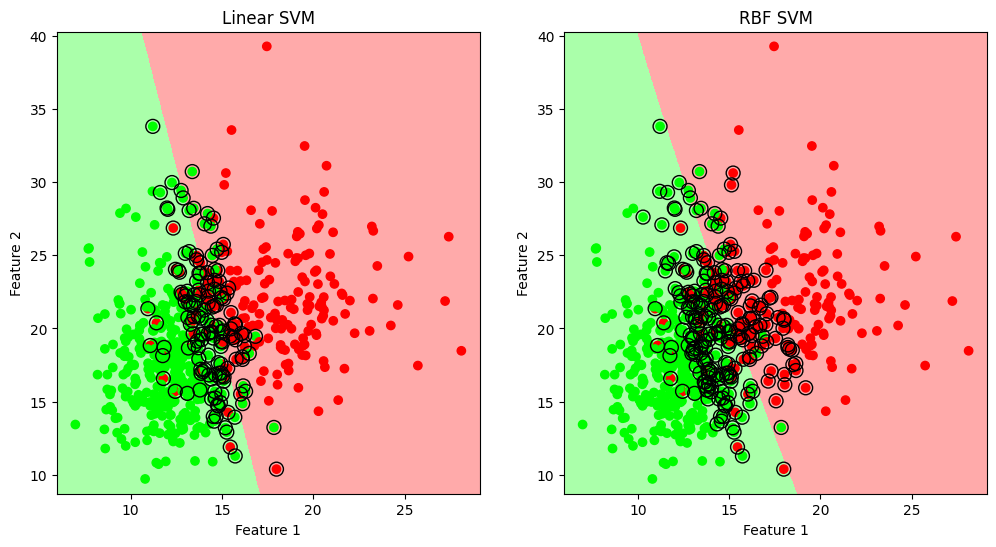
\includegraphics[scale=0.4]{download.png}
	\caption{线性核函数与高斯核函数相对比}
	\label{bfgs}
\end{figure}
{\hei 实验结果表明,高斯核函数在本数据集上的表现优于线性核函数,具有更高的准确率,这说明高斯核函数能够更好地捕捉数据的非线性特征,提高分类性能。}

\chapter{\hei 支持向量机算法的应用}
支持向量机算法可以有效地处理高维数据和非线性数据,具有很高的准确性和泛化能力,在模式识别、生物信息学、金融预测、医学检测、计算机视觉、文本分类等领域都有广泛应用。
\section{模式识别}
支持向量机在模式识别领域的应用最广泛,已成功地解决了诸如手写体、图像处理、语音识别等许多识别和分类问题。

在手写字体识别方面,当采用5层神经网络算法时,其识别的错误率为5.1\%;贝尔实验室\cite{cortes1995support}最先将SVM应用于手写字体识别研究,选取三种不同的核函数时,得到的误识率分别为4.0\%,4.1\%和4.2\%,可看出支持向量机方法比神经网络算法具 有更好的分类准确性。

在人脸识别方面,由于人脸图像存储和支持向量机训练需要大量的存储空间,周志明[15]等人将小波变换与支持向量机相结合,由小波变换提取人脸特 征,减小特征向量维数并将其输入到支持向量机中,并结合最近邻分类器进行分类,提高了分类器的鲁棒性和分类精度。